%&LaTeX
\batchmode
\documentclass{article}
\usepackage{setspace}
\usepackage{graphicx}
\usepackage{hyperref}
\def\R2Lurl#1#2{\mbox{\href{#1}{\tt #2}}}
\newcommand{\tab}{\hspace{5mm}}


\begin{document}


\begin{center}

\begin{spacing}{1.5}
\textbf{{\huge STIR \\
General Overview}}\\
\textbf{Kris Thielemans}\\
\textbf{\textit{version 2.3}}


\end{spacing}

\end{center}

\tableofcontents 
%\section{Contents}
%\begin{itemize}
%\item Overview
%\item A bit more detail on the library
%\item Reconstruction algorithms currently distributed
%  \begin{itemize}
%  \item Ordered Subsets Maximum A Posteriori using the One Step Late algorithm
%  \end{itemize}
%\item Optimisation
%\item Software testing strategy
%\item Currently supported systems
%  \begin{itemize}
%  \item  Computing platforms
%    \begin{itemize} 
%    \item Serial versions of algorithms
%    \item Parallel versions of algorithms
%    \end{itemize}
% \item Compilers
% \item PET scanners
% \item File formats
% \end{itemize}
%\item References
%\end{itemize}


\section{
Disclaimer}
Many names used below are trademarks owned by various companies. They are
is fully acknowledged, but not explicitly stated.

\section{
Overview}

STIR (\textit{Software for Tomographic Image Reconstruction}) is Open 
Source software (written in C++) consisting of classes, functions 
and utilities for 3D PET image reconstruction, although it is 
general enough to accommodate other imaging modalities. An overview
of STIR 2.x is given in [Thi12], which you ideally refer to in your paper.

STIR consists of 2 parts. 
\begin{itemize}
\item
A library providing building blocks for image and projection 
data manipulation and image reconstruction.
\item
Applications using this library including basic image manipulations, 
file format conversions and of course image reconstructions.
\end{itemize}

The library has been designed so that it can be used for many 
different algorithms and scanner geometries. The library contains 
classes and functions to run parts of the reconstruction in parallel 
on distributed memory architectures, although these are not distributed 
yet. This will enable the software to be run not only on single 
processors, but also on massively parallel computers, or on clusters 
of workstations. \\
STIR is portable on all systems supporting the GNU C++ compiler 
or MS Visual C++ (or hopefully any ANSI C++ compliant compiler). 
The library is fully documented.\\
The object-oriented features make this library very modular and 
flexible. This means that it is relatively easy to add new algorithms, 
filters, projectors or even a different type of image discretisation. 
It is even possible to select at run-time which version of these 
components you want to use.\\
The software is \textbf{freely available} for downloading under the 
GNU LPGL (the library) or GNU GPL (the applications) license, 
see the 'Registration' section of our web-site. \\
\textbf{It is the hope of the collaborators of the STIR project that 
other researchers in the PET community will use this library 
for their own work, extending it and making their work available 
as well.} Please subscribe to some of our mailing 
lists if you are interested. \\
In its current status, the software is mainly a research tool. 
It is probably not friendly enough to use in a clinical setting. In any 
case, \textbf{STIR should not be used to generate images for diagnostic
purposes}, as there is no warranty, and most definitely no FDA approval




\section{
A bit more detail on the library}

The STIR software library uses the object-oriented features of 
C++:

\begin{itemize}

\item self-contained objects hide implementation details from the user 
(\textit{encapsulation});
\item specialisation of concepts is implemented with hierarchies 
of classes (\textit{inheritance});
\item conceptually identical operations are implemented using 
functions with identical names (\textit{polymorphism}).
\end{itemize}

The building block classes included in this library are as follows:

\begin{itemize}
\item information about the data (scanner characteristics, study type, 
algorithm type, etc.);
\item multi-dimensional arrays (any dimension) with various 
operations, including numeric manipulations;
\item reading and writing (I/O) data in Interfile format (for 
which a 3D PET extension is proposed), reading of GE Advance 
sinogram data, limited reading and writing of ECAT6 and ECAT7 
and conversion between ECAT6 and Interfile;
\item classes of projection data (complete data set, segments, 
sinograms, viewgrams) and images (2D and 3D);
\item various filter transfer functions (1D, 2D and 3D);
\item forward projection and backprojection operators;
\item classes for sparse projection matrices, both for on-the-fly 
computation and pre-stored;
\item trimming and zooming utilities on projection and image 
data;
\item classes for scatter estimation
\item classes for normalisation and attenuation correction
\item classes for iterative reconstruction algorithms;
\item some classes for kinetic modelling and parametric imaging
\item stream-based classes for message passing between different 
processes, built on top of MPI
\end{itemize}

Examples of hierarchies are given in the following figures:
\begin{figure}[htbp]
\begin{center}
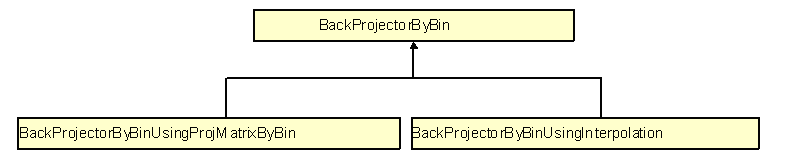
\includegraphics[width=5.667in, height=1.137in]{graphics/STIR-general-overviewFig1}
\caption{Current hierarchy for back projectors.}
\end{center}
\end{figure}


\begin{figure}[htbp]
\begin{center}
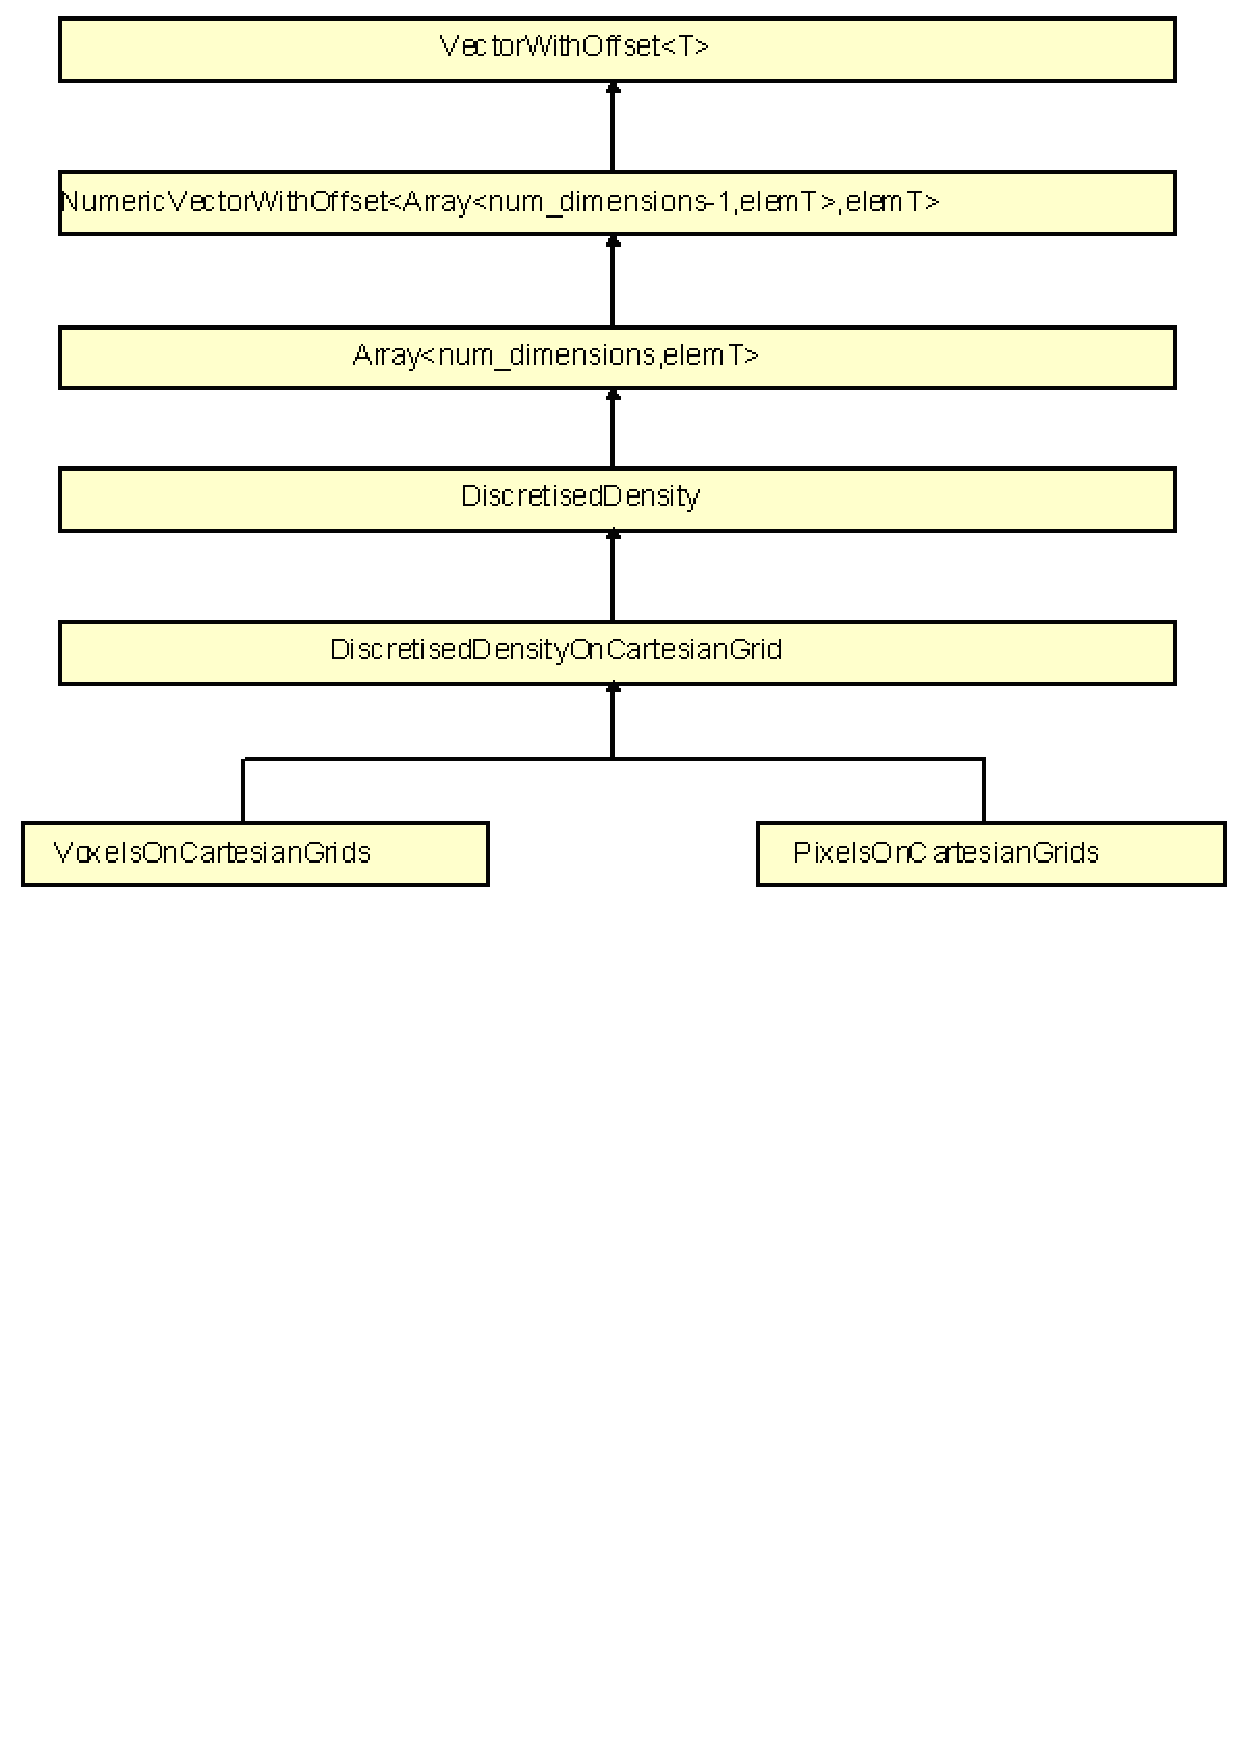
\includegraphics[width=4.100in, height=2.984in]{graphics/STIR-general-overviewFig2}
\caption{Current image hierarchy}
\end{center}
\end{figure}

These figures are extracted from the documentation which is available 
in HTML, LaTeX and PDF. This documentation is generated automatically 
from the source files of the library using the \R2Lurl{http://www.doxygen.org/ }{doxygen} 
tool. This means that it requires minimal effort to keep the 
documentation up-to-date.

The advantages of such a library are (a) modularity and flexibility 
of the reconstruction building blocks to implement new reconstruction 
algorithms, (b) possibility to compare analytic and iterative 
methods within a common framework, (c) the possibility to use 
the same software implementation of the building blocks to perform 
image reconstruction on different scanner geometries and (d) 
independence of the computer platform on which the software runs.



\section{
Reconstruction algorithms currently distributed}

\subsection{FBP}
Optionally with SSRB first.

\subsection{3DRP}
The 3DRP [Kin89] algorithm is often considered the 'reference' 
algorithm for 3D PET. It is a 3D FBP algorithm which uses reprojection 
to fill in the missing data.

\subsection{
Ordered Subsets Maximum A Posteriori using the One Step Late 
algorithm}

The Expectation Maximization (EM) algorithm [She82] as well as 
its accelerated variant OSEM (Ordered Set Expectation Maximization) 
[Hud94] are iterative methods for computing the maximum likelihood 
estimate of the tracer distribution based on the measured projection 
data. Their benefits have been examined in various reports. Notably, 
it has been found (e.g. [Rea98b]) that 3D OSEM can produce images 
of higher quality, in terms of both resolution and contrast, 
than analytic algorithms of common commercial use such as the 
reprojection (3DRP) algorithm [Kin89].

One drawback of OSEM is its tendency to develop noise artefacts 
with increasing iterations. As a remedy, various modifications 
of the image updating mechanism have been investigated for EM 
and OSEM to drive the image estimate sequence toward a smoother 
limit. These include the addition of a smoothing step between 
iterations (e.g. [Sil90]) and Bayesian methods which incorporate 
prior information about the smoothness of the object to be reconstructed 
(e.g. [Gem84], [Heb89]).


\begin{spacing}{1.5}
\textit{Filtering}


\end{spacing}

Different types of filtering strategies are possible (and implemented 
in STIR). Post-filtering is the most common choice. Inter-iteration 
filtering filters the image after every (sub)iteration, or at 
a lower frequency. It probably was poineered in [Sil90] for EMML 
where it was called Expectation Maximisation Smoothing (EMS). 
Inter-update filtering is similar. Forward
projection of the current image iterate is done first in order to
compute the usual ML-EM image of multiplicative weights. These weights are
then applied to a filtered version of this image to generate the next
iterate, for further details see [Jac99].\\
See [Sli98] for a comparison between post- and inter-iteration 
filtering, where it is claimed that both give similar results. 
[Mus01a],[Mus01b] discusses resolution properties of EMS and 
shows that it can generate resolution which is object-dependent.



\begin{spacing}{1.5}
\textit{Maximum A Posteriori (Bayesian)}


\end{spacing}

Bayes theorem allows the introduction of a prior distribution 
into the reconstruction process that describes properties of 
the unknown image. Maximisation of this \textit{a posteriori} probability 
over a set of possible images results in a MAP estimate. Priors 
may be added one by one into the estimation process, assessed 
individually, and used to guarantee a fast working implementation 
of preliminary versions of the algorithms [LAL93], [LAN90].

Markov Random Fields (MRF) are used to describe the relationship 
between adjacent pixels. Gibbs Random Fields (GRF) represent 
a subset of MRFs which originate from statistical physics, where 
the problem is to estimate large scale properties of a lattice 
system from its local properties. Hence, the Bayesian model can 
utilise a Gibbs prior to describe the spatial correlation of 
neighbouring regions as was first suggested by Geman et al. in 
1984 [GEM84]. The Gibbs prior is controlled by three parameters: 
one determines the overall weight placed on the prior in the 
reconstruction process, the two others affect the relative smoothing 
of noise versus edges in the reconstructed image estimates. Their 
derivative will act as a penalty term that enforces conditions 
required by the prior.

The STIR executable OSMAPOSL allows to run a MAP algorithm 
known as the One Step Late [Gre90] modification of MLEM obtained 
by multiplying the ML-EM equation by a factor that uses the derivative 
of an \textit{energy function}. This algorithm works fine 
for small weights of the prior term, however becomes unstable 
for larger values. 

As prior we currently only distribute the ``quadratic penalty'', i.e. a
Gibbs prior with a qudratic potential function, and a generalisation of the 
Median Root prior (MRP) [Ale97]. In the MRP case, the assumption 
is that the desired image is locally monotonic, and that the 
most probable value of the pixel is close to the local median. 
MRP has shown very interesting properties in terms of noise reduction, 
quantitative accuracy, and convergence, see [Bett01]. Our (obvious) 
generalisation consists in allowing to use other filters than 
the Median. Other priors can easily be added with some coding. 


\subsection{OSSPS}
An implementation of OSSPS [Ahn03] is included since STIR version 2.1. 
This algorithm is designed for penalised reconstruction (MAP). When used
with a decreasing relaxation constant, it is theoretically convergent [Ahn03].
In practice, it works best when initialised fairly close to the final solution,
and when a non-zero background term (e.g. randoms or scatter) is present.

As OSSPS is implemented using the same framework as OSMAPOSL, it is possible
to use inter-iteration filtering for OSSPS. Interestingly, 
[Mus01a],[Mus01b] showed that when used with spatially uniform filtering,
this algorithm has nearly object-independent
resolution properties, in contrast to EMS.

\subsection{Other}

We distribute an implementation of FORE  [Def97]. It is an efficient 
rebinning algorithm to reduce the data-size from 3D-PET to 2D-PET. 

PARAPET code for 
Ordered Subsets Conjugate Barrier (OSCB) [Mar99] exists but needs
a bit of work to convert to STIR. Please let us know if you 
want to help.
 
With respect to dynamic and gated imaging
techniques, we have direct estimation of Patlak
parameters [Tso08] (using Parametric OSMAPOSL or OSSPS).
We plan to release motion compensated image reconstruction [Thi06] as
implemented by Tsoumpas et al [Tso11].

\section{
Optimisation}

Optimisation of the implementation for any particular hardware 
architecture or intercommunication topology is not attempted 
in STIR. Therefore the main goals of optimisation and parallelisation 
were:
\begin{itemize}
\item to allow evaluation of the reconstruction algorithms to be 
carried out within a reasonable time frame; indeed, the parallel 
versions of the reconstruction algorithms have been extensively 
used during algorithm evaluation;
\item to improve clinical usability of the results of the project; 
this has been achieved by providing parallel implementations 
of the algorithms that allow clinicians to run the selected variety 
of reconstruction algorithms even for very large PET-scanners 
on MIMD-parallel systems without any knowledge of parallel computing.
\end{itemize}


\section{
Software testing strategy}

As the STIR software library is quite extensive, it was essential 
to test its components separately. Due to its modular design, 
it was possible to have a fairly comprehensive test strategy.

Nearly all basic building blocks have their own test class, checking 
a lot of test cases. Running of these tests is fully automated.

The projectors have in a first stage been tested interactively. 
For the forward projector this consisted in forward projecting 
various images and comparing with the known result. Results were 
also compared with an independent implementation of a ray-tracing 
forward projection. For the interpolating backprojector the test 
which revealed most problems was to backproject uniform data, 
as this should give (locally) uniform images. The resulting image 
was also calculated analytically and compared with the building 
blocks result. Finally, different groups of symmetry were used, 
cross-checking different parts of the code. Once these tests 
confirmed properly working projectors, our main strategy consisted 
in checking results of new versions with the established results.

Aside from these checks, all algorithms can run in a debugging 
mode where assertions  check consistency and validity.

Finally, the web-site also provide the \texttt{recon\_test\_pack}.
The distributed script contains consistency checks on the reconstruction
(forward simulation followed by reconstruction with various algorithms) and
a number of data-sets and expected end-results.


\section{
Currently supported systems}

These are the systems we tested our software on. We think that 
it will work in other cases as well with minor tuning. Experience 
will tell\dots 



\subsection{
Computing platforms}


\subsubsection{
Serial versions of algorithms}
A lot of STIR was developed kust before 2000. Therefore, the code
contains in various places work-arounds for deficient C++ compilers
(e.g. GNU g++ 2.95.2 or Microsoft Visual C++ 6.0 service pack 3). 
However, we are no longer
testing STIR on such older systems. It might be possible to revive this,
but we strongly recommend that you get a recent compiler instead.
\begin{itemize}
\item 
Intel based PCs using Windows XP or higher (NT probably still works if you
find a compiler for it). These were tested with Microsoft Visual C++ 2003, 2005 up to
Visual Studio 2010,
and various GNU g++ versions (up to at least 4.5.3) via CYGWIN (http://cygwin.com).
\item 
Linux using GNU g++ (from 3.5 to 4.6).
Intel's C++ compiler 12.1.0  works fine (tested on Linux), older versions had some problems with the Fourier transform code but the reconstruction itself was fine.
\item
MacOS using GNU g++.
\end{itemize}
However, people run STIR on various other systems, including Solaris. Please
check the mailing lists.

\textbf{Warning}: 
We currently have a problem 
in the incremental backprojection routines due to different rounding 
of floating point calculations on Sparc, HP and Opteron processors. 
Thanks to a fix of Bing Bai this problem might have disappeared on your processor, but it is still there on recent 64-bit processors.
You will find out if this problem still exists when you run the 
recon\_text\_pack available on the STIR web-site. Please let us know.
See the User's Guide for how to use another backprojector.


\subsubsection{
Parallel versions of algorithms}
\begin{itemize}
\item a parallel version of \texttt{OSMAPOSL} and \texttt{OSSPS} using MPI 
\item a threaded version of FBP2D using OPENMP, but for most systems, there is no performance gain.
\end{itemize}




\subsection{
PET scanners}
\begin{itemize}
\item 
GE Advance, Discovery LS, Discovery ST, Discvoery STE, Discovery RX,
Discovery 600 
\item 
PRT-1 
\item 
ECAT 921, 931, 953, 951, 962, 966 (and most other ECAT systems) 
\item 
HRRT apparently works as well
\item Philips Allegro (using its convention of having a ``virtual'' extra crystal to cover the gaps).
\end{itemize}

Other cylindrical PET scanners can easily be added. This can be done
without modifying the code (see the Wiki).


\subsection{
File formats}
\begin{itemize}
\item 
An extension of the Interfile standard (see the ''Other info'' section of the STIR website.)
\item 
The commercial AnalyzeAVW library from the BIR, Mayo University, can be used
to read images via a conversion utility.
\item 
GE Advance VOLPET sinogram format, but for reading only (with 
very limited support for the header). If you have a research contract with GE,
you might be able to get a STIR extension to read Discovery ST, STE and RX data in both 
VOLPET and RDF format.
\item 
ECAT 7 matrix format for reading only (for reading multiple
frames/gates, an Interfile 
header has to be created using a utility we provide). Single 
frame/gate/bed images can be directly read or written. Single 
frame/gate/bed sinograms can be directly read.
However, this file format needs the ECAT Matrix library (developed 
previously by M. Sibomana and C. Michel at Louvain la Neuve, Belgium).
This library is no longer maintained however.
\item 
ECAT 6 matrix format was supported in previous version of STIR, but
is currently broken on some systems (probably due to a bug in the ECAT 
MATRIX library for ECAT 6). ECAT6 was supported by using conversion 
utilities to and from 
Interfile. Single frame/gate/bed images could be directly read 
or written.
\end{itemize}

See the User's Guide for more detail on the supported file formats.\\
In addition, a separate set of classes is avalailable
to read list-mode 
data. Only a few scanners are currently supported (such as the 
ECAT HR+ and HR++), although it should not be too difficult to 
add your own (if you know the list-mode file format!). 



\section{
References}

{[}Ale97{]} Alenius S and Ruotsalainen U \textbf{(1997)} Bayesian image 
reconstruction for emission tomography based on median root prior. \textit{European 
Journal of Nuclear Medicine} , Vol. 24 No. 3: 258-265.\\
{[}Ahn03{]}S. Ahn, J. A. Fessler. \textbf{2003}
Globally convergent image reconstruction for emission tomography using relaxed ordered subsets algorithms. 
\textit{IEEE Trans. Med. Imag.}, 22(5):613-626. \\
{[}Bar97{]} Barrett H, White T and Parra L C \textbf{(1997)} List mode 
likelihood. \textit{J. Opt. Soc. Am.}, A 14: 2914-2923.\\
{[}Ben99a{]} Ben-Tal A, Margalit T and Nemirovski A \textbf{(1999)} The 
ordered subsets mirror descent optimization method with application 
to tomography. \textit{Research report \#2/99, March 1999, MINERVA 
Optimization Center, Faculty of Industrial Engineering and Management, 
Technion -- Israel Institute of Technology}.\\
{[}Ben99b{]} Ben-Tal A and Nemirovski A \textbf{(1999)} The conjugate 
barrier method for non-smooth, convex optimization. R\textit{esearch 
report \#5/99, October 1999, MINERVA Optimization Center, Faculty 
of Industrial Engineering and Management, Technion -- Israel Institute 
of Technology.}\\
{[}Bett01{]} V. Bettinardi, E. Pagani, M. C. Gilardi, S. Alenius, 
K. Thielemans, M. Teras and F. Fazio \textbf{(2001)}, Implementation 
and evaluation of a 3D one-step late reconstruction algorithm 
for 3D positron emission tomography brain studies using median 
root prior, \textit{Eur. J. Nucl. Med, in press.}\\
{[}Dau86{]} Daube-Witherspoon M E and Muehllener G \textbf{(1986)} An 
iterative space reconstruction algorithm suitable for volume 
ECT. \textit{IEEE Trans. Med. Imaging}, vol. MI-5: 61-66.\\
{[}Def97{]} Defrise M, Kinahan P E, Townsend D W, Michel C, Sibomana 
M and Newport D F \textbf{(1997)} Exact and approximate rebinning 
algorithms for 3-D PET data. \textit{IEEE Trans. Med. Imag}ing, MI-16: 
145-158.\\
{[}Gem84{]} Geman S and Geman D \textbf{(1984)} Stochastic relaxation, 
Gibbs distributions, and the Bayesian restoration of images. \textit{IEEE 
Trans PAMI}, 6: 721-741.\\
{[}Gem85{]} Geman S. and McClure D \textbf{(1985)} Bayesian image analysis: 
an application to single photon emission tomography. \textit{in Proc. 
American Statistical Society, Statistical Computing Section (Washington, 
DC)} 12-18.\\
{[}GEMS{]} General Electric Medical Systems homepage {\underline {http://www.gems.com}}.\\
{[}Gre90{]} Green P J \textbf{(1990)} Bayesian reconstruction from emission 
tomography data using a modified EM algorithm. \textit{IEEE Trans. 
Med. Imaging}, MI-9: 84-93.\\
{[}Heb89{]} Hebert T J and Leahy R M \textbf{(1989)} A generalized EM 
algorithm for 3-D Bayesian reconstruction from Poisson data using 
Gibbs priors. \textit{IEEE Trans. Med. Imaging}, MI-8: 194-202.\\
{[}Her80{]} Herman G T \textbf{(1980)} Image Reconstruction from Projections: 
The fundamentals of Computational Tomography. \textit{Academic Press, 
New York}.\\
{[}Hud94{]} Hudson H M and Larkin R S \textbf{(1994)} Accelerated image 
reconstruction using ordered subsets of projection data. \textit{IEEE 
Trans. Med. Imaging}, MI-13: 601-609.\\
{[}Jac99{]} Jacobson M, Levkovitz R, Ben-Tal A, Thielemans K, Spinks 
T, Belluzzo D, Pagani E, Bettinardi V, Gilardi M C, Zverovich 
A and Mitra G \textbf{(1999)} Enhanced 3D PET OSEM Reconstruction 
using inter-update Metz filters. in Press in \textit{Phys. Med. Biol.}\\
{[}Kin89{]} Kinahan P E and Rogers J G \textbf{(1989)} Analytic 3D image 
reconstruction using all detected events. \textit{IEEE Trans. Nucl. 
Sci.}, 36: 964-968. \\
{[}Lal93{]} Lalush D S and Tsui M W \textbf{(1993)} A general Gibbs prior 
for Maximum a posteriori reconstruction in SPET. \textit{Phys. Med. 
Biol.}, 38: 729-741.\\
{[}Lan90{]} Lang K \textbf{(1990)} Convergence of EM Image reconstruction 
algorithms with Gibbs smoothing. \textit{IEEE Trans. Med. Imaging}, 
MI-9: 4.\\
{[}Mus01a{]} S. Mustafovic, K.Thielemans, D. Hogg and P. Bloomfield \textbf{(2001)} 
\textit{Object Dependency of Resolution and Convergence Rate in OSEM 
with Filtering,} proc. of 3D-2001 conference.\\
{[}Mus01b{]} S. Mustafovic, K.Thielemans, D. Hogg and P. Bloomfield \textbf{(2001)} \textit{Object 
Dependency of Resolution and Convergence Rate in OSEM with Filtering}, 
proc. of IEEE Medical Imaging Conf. 2001.\\
{[}Mar99{]} Margalit T, Gordon E, Jacobson M, Ben-Tal A, Nemirovski 
A, Levkovitz R \textbf{(1999)} The ordered sets mirror descent and 
conjugate barrier optimization algorithms adapted to the 3D PET 
reconstruction problem. Submitted to \textit{IEEE Trans. Med. Im.}aging.\\
{[}Nem78{]} Nemirovski A and Yudin D \textbf{(1978)} Problem complexity 
and method efficiency in optimization. \textit{Nauka Publishers, 
Moscow, 1978 (in Russian); English translation: John Wiley \& 
Sons, 1983}.\\
{[}Rea98a{]} Reader A J, Erlandsson K, Flower M A and Ott R J \textbf{(1998)} 
Fast accurate iterative reconstruction for low statistics positron 
volume imaging. \textit{Phys. Med. Biol.}, 43: 835-846.\\
{[}Rea98b{]} Reader A J, Visvikis A, Erlandsson K, Ott R J, and Flower 
M A \textbf{(1998)} Intercomparison of four reconstruction techniques 
for positron volume imaging with rotating planar detectors. \textit{Phys. 
Med. Biol.}, 43: 823-34.\\
{[}She82{]} Shepp L A and Vardi Y \textbf{(1982)} Maximum likelihood reconstruction 
for emission tomography. \textit{IEEE Trans. Med. Imaging}, 1: 113-122.\\
{[}Sil90{]} Silverman B W, Jones M C, Wilson J D, and Nychka D W \textbf{(1990)} 
A smoothed EM approach to indirect estimation problems, with 
particular reference to stereology and emission tomography. \textit{J. 
Roy. Stat. Soc}., 52: 271-324.\\
{[}Sli98{]} Slijpen E T P, Beekman F J \textbf{(1998)} Comparison of post-filtering 
and filtering between iterations for SPECT reconstruction. \textit{in 
Proc. IEEE Nucl. Sci. Symp. and Med. Imaging Conf.}, 2: 1363-6.\\
{[}Thi06{]} Thielemans, K., Manjeshwar, R. M., Xiaodong T., and Asma E.
\textbf{(2006)}, Lesion detectability in motion compensated
image reconstruction of respiratory gated PET/CT. \textit { 2006 IEEE
Nuclear Science Symposium and Medical Imaging Conference} 3278-3282.
{[}Thi99{]} Thielemans K, Jacobson M W, Belluzzo D \textbf{(1999)} On 
various approximations for the projectors in iterative reconstruction 
algorithms for 3D-PET. \textit{in Proceedings of the 3D99 Conference, 
Egmond Aan Zee}, (June 1999): 232-235.
[Thi12] Kris Thielemans, Charalampos Tsoumpas, Sanida Mustafovic, Tobias Beisel, Pablo Aguiar, Nikolaos Dikaios, and Matthew W Jacobson,
\textit{STIR: Software for Tomographic Image Reconstruction Release 2},
Physics in Medicine and Biology, 57 (4), 2012 pp.867-883.
{[}Tso08{]} Tsoumpas C, Turkheimer F E, Thielemans K \textbf{(2008)},
Study of direct and indirect parametric estimation methods of linear
models in dynamic positron emission tomography. \textit{Med. Phys.} 35(4):
p. 1299-1309.
{[}Tso11{]} Tsoumpas, C., et al \textbf{(2011)}, The effect of
regularisation in motion compensated image reconstruction. \textit { IEEE
Nucl Sci Symp Med Imaging Conf }.



\end{document}
